\newpage

\pagestyle{fancy}
\lhead{\textsc{Chapter 2.Gestion de projet et méthodologie SCRUM}}
\renewcommand{\headrulewidth}{0.5pt}
\renewcommand{\footrulewidth}{0.5pt}

\chapter{Gestion de projet et méthodologie SCRUM}\setlength{\headheight}{28pt}
\label{ch2}
\minitoc
\newpage

\section{Introduction}
Ce chapitre présente la démarche méthodologique adoptée pour la réalisation du projet décisionnel BIOSPHERE. Dans le cadre d’un projet combinant Business Intelligence, Data Engineering et Data Science, il est essentiel de mettre en place une organisation rigoureuse permettant d’assurer une bonne gestion des besoins métier, une planification efficace des tâches ainsi qu’une adaptation continue aux évolutions fonctionnelles et techniques.\\
Afin de répondre à ces exigences, une approche Agile basée sur la méthodologie Scrum a été choisie. Cette méthode a permis de structurer le projet en plusieurs sprints, de prioriser les fonctionnalités selon leur valeur métier et d’assurer un suivi progressif de l’avancement des travaux.\\
Ce chapitre commence par l’analyse des besoins fonctionnels et non fonctionnels du système, suivie de la définition des principaux indicateurs clés de performance (KPI) utilisés pour l’analyse décisionnelle. Ensuite, il présente les principes de la méthodologie Scrum adoptée, les rôles attribués, les User Stories ainsi que la planification des sprints à l’aide d’un diagramme de Gantt. Enfin, une modélisation UML à travers un diagramme de cas d’utilisation est proposée afin de représenter les interactions entre les différents acteurs et le système décisionnel développé.
\section{Section 1 : Recueil des besoins}
Le recueil des besoins est la première étape de tout projet de systèmes d'information. Son objectif est de formaliser les exigences fonctionnelles et non fonctionnelles nécessaires au développement d'une solution, en s'appuyant sur des entretiens avec les parties prenantes métier qui sont les responsables de l’entreprise biosphère dans notre cas.\\
Cette phase d'analyse a été menée avant le démarrage du développement car elle vise à identifier les attentes fonctionnelles et techniques du système décisionnel dans une première étape puis les mettre en place.
\subsection{Besoins fonctionnels}
Un besoin fonctionnel décrit ce que le système doit faire tel que les services, traitements et comportements qu'il doit offrir pour répondre aux exigences métier des utilisateurs. Il exprime une fonctionnalité concrète, observable et testable.\\
Selon Sharda, Delen \& Turban: « Les besoins fonctionnels d'un système décisionnel décrivent les capacités analytiques que la solution doit fournir aux utilisateurs, notamment la collecte, l'intégration, l'analyse et la présentation des données sous forme d'indicateurs, de rapports et de tableaux de bord interactifs. » \cite{Sharda2024}
\subsubsection{Tableau de bord décisionnel unifié}
Les utilisateurs (directeur, managers de site) ont le besoin d'une vue synthétique de la performance globale, accessible en quelques clics et adaptée à leur profil. Ce besoin couvre :
\begin{itemize}
    \item Un tableau de bord consolidant les KPI principaux et couvre les principaux départements : ventes, achats, profit, marge, stock
    \item Une segmentation automatique par site lorsque pertinent
    \item Un tableau de bord dynamique
\end{itemize}
\subsubsection{Page Business Intelligence détaillée}
Un second besoin consiste à disposer d'une page dédiée à l'analyse approfondie des KPI, avec :
\begin{itemize}
    \item Des cartes KPI interactives couvrant ventes, achats, profit, marge, stock total, stock disponible, articles en rupture
    \item Une lecture adaptée au rôle de l'utilisateur (Directeur, Manager\_TN, Manager\_SFX)
    \item Un contexte d'affichage (année active détectée automatiquement, date de cutoff stock)
\end{itemize}
\subsubsection{Faire une Prévision de Stock }
Un besoin critique consiste à anticiper les ruptures de stock et estimer les niveaux futurs. Cela demande :
\begin{itemize}
    \item Un système de priorité des produits à risque (critique, moyen, normal)
    \item Un tableau des produits à surveiller en priorité
\end{itemize}
\subsubsection{Page Alertes automatiques}
Les responsables métier ont besoin d'un système d'alertes capable de :
\begin{itemize}
    \item Générer des alertes stock en fonction de règles prédéfinies
    \item Classer les alertes par sévérité (critique, moyen)
    \item Afficher un historique des alertes avec statuts
    \item Filtrer par produit, site, priorité et statut
    \item Envoyer automatiquement une notification email pour les alertes critiques
\end{itemize}
\subsubsection{Gestion des accès et authentification}
La solution doit fournir :
\begin{itemize}
    \item Un système d'authentification local sécurisé (login/mot de passe)
    \item Trois rôles disponibles : Directeur (accès global), Manager\_TN (site Tunis), Manager\_SFX (site Sfax)
    \item Une restriction automatique des vues et des données selon le rôle
\end{itemize}


\begin{table}[H]
\centering
\caption{Récapitulatif des besoins fonctionnels}
\renewcommand{\arraystretch}{1.1}
\label{tab:ch2:besoins_fonctionnels}
\small
\begin{tabular}{|p{12cm}|}
\hline
\multicolumn{1}{|c|}{\textbf{Besoins fonctionnels}} \\
\hline
Développer des Dashboard Power BI pour les ventes, achats et stocks \\
\hline
Intégrer une gestion des rôles et des accès (RLS) \\
\hline
Suivre les KPI et indicateurs décisionnels \\
\hline
Prédire les risques de rupture de stock \\
\hline
Prévoir les niveaux futurs de stock \\
\hline
Générer automatiquement des alertes critiques \\
\hline
Intégrer les modèles BI et IA dans une application décisionnelle \\
\hline
\end{tabular}
\end{table}

\subsection{Besoins non-fonctionnels}
Les besoins non-fonctionnels définissent les nécessités de qualité et les contraintes techniques auxquelles le système doit répondre afin d’assurer le bon fonctionnement, la sécurité, la performance et la facilité d’utilisation.

Selon Chen, Chiang \& Storey : « Dans un projet de Business Intelligence et de Data Science, les besoins non-fonctionnels englobent les exigences de scalabilité, de disponibilité, de gouvernance des données et de sécurité des accès, qui sont essentielles pour assurer la pérennité et la robustesse de la solution décisionnelle. » \cite{Chen2024}(Chen, 2024)
\subsubsection{Performance et disponibilité}
\begin{itemize}
    \item Disponibilité : le système doit fonctionner en local, indépendamment d'une connexion internet
    \item Scalabilité : la solution doit pouvoir traiter les données de 3 à 5 ans sans dégradation notable
\end{itemize}
\subsubsection{Sécurité et gouvernance des données}
\begin{itemize}
    \item Les données relatives à un site ne doivent pas être accessibles aux utilisateurs d'un autre site.
\end{itemize}
\begin{table}[H]
\centering
\caption{Récapitulatif des besoins non fonctionnels}
\renewcommand{\arraystretch}{1.1}

\begin{tabular}{|p{12cm}|p{7cm}|}
\hline

\multicolumn{1}{|c|}{\textbf{Besoins non fonctionnels}} \\
\hline

Assurer une séparation claire entre les couches techniques \\
\hline

Garantir la reproductibilité de l’environnement avec Docker \\
\hline

 Assurer la sécurité et le contrôle des accès utilisateurs \\
\hline

Permettre une actualisation automatique quotidienne des données \\
\hline

Assurer de bonnes performances de traitement \\
\hline

Garantir une visualisation claire et exploitable des données \\
\hline

Assurer la stabilité et la portabilité de l’environnement technique \\
\hline

\hline

\end{tabular}
\end{table}
\subsection{Liste des KPI décisionnels avec formules}
Après l’étape de l’analyse des besoins, il devient essentiel de définir des indicateurs clés de performance (KPI) afin d’évaluer l’efficacité des actions mises en place et de mesurer l’atteinte des objectifs fixés. Les KPI permettent de traduire les besoins identifiés en données mesurables et exploitables, facilitant ainsi le suivi de la performance, la prise de décision et l’amélioration continue. Dans cette perspective, la section suivante présente les principaux indicateurs retenus pour évaluer les résultats du projet et analyser son impact de manière objective et structurée.
%================= TABLEAU KPI COMPLET =================

{\footnotesize
\renewcommand{\arraystretch}{1.3}
\setlength{\tabcolsep}{3pt}


\begin{longtable}{|p{2cm}|p{1.8cm}|p{2.8cm}|p{2.2cm}|p{6cm}|}

\caption{Récapitulatif des KPI} \\

\hline
\multicolumn{1}{|c|}{\textbf{Catégorie}} & 
\multicolumn{1}{c|}{\textbf{KPI}} & 
\multicolumn{1}{c|}{\textbf{Formule de calcul}} & 
\multicolumn{1}{c|}{\textbf{Source de données}} & 
\multicolumn{1}{c|}{\textbf{Description et utilité}} \\
\hline
\endfirsthead

\hline
\multicolumn{1}{|c|}{\textbf{Catégorie}} & 
\multicolumn{1}{c|}{\textbf{KPI}} & 
\multicolumn{1}{c|}{\textbf{Formule de calcul}} & 
\multicolumn{1}{c|}{\textbf{Source de données}} & 
\multicolumn{1}{c|}{\textbf{Description et utilité}} \\
\hline
\endhead

\hline
\endfoot

%================= KPIs STOCK =================

\multicolumn{5}{|c|}{\cellcolor{gray!25}\textbf{LES KPIs DU STOCK}} \\
\hline

Niveau de stock & Stock total (unités) & SUM (clipped\_stock) & Fact\_Stock + reconstruction & \textbf{Description :} Quantité totale de produits disponibles en stock après correction des valeurs négatives. \newline \textbf{Utilité :} Permet d'avoir une vision globale du niveau de stock et d'éviter les ruptures ou le surstockage. \\
\hline

Disponibilité & Stock disponible & SUM(IF([Stock] > 0, [Stock], 0)) & Fact\_Stock & \textbf{Description :} Volume de stock réellement disponible pour la vente (exclut les stocks négatifs). \newline \textbf{Utilité :} Indique la capacité réelle à satisfaire les commandes clients immédiatement. \\
\hline

Ruptures & Nombre d'articles en rupture & COUNT(IF([Stock] $\leq$ 0, 1)) & Fact\_Stock & \textbf{Description :} Nombre de produits dont le stock est nul ou négatif. \newline \textbf{Utilité :} Identifie les produits indisponibles qui impactent les ventes et la satisfaction client. \\
\hline

Valeur & Valeur totale du stock & SUM([Stock] * PUHT) & Fact\_Stock + Dim\_Produit & \textbf{Description :} Valeur monétaire totale du stock basé sur le prix unitaire. \newline \textbf{Utilité :} Permet d'évaluer l'immobilisation financière et d'optimiser la trésorerie. \\
\hline

Rotation & Taux de rotation des stocks & [CA] / [Stock moyen] & Fact\_Vente + Fact\_Stock & \textbf{Description :} Nombre de fois où le stock est renouvelé sur une période donnée. \newline \textbf{Utilité :} Mesure l'efficacité de la gestion des stocks et la rapidité d'écoulement des produits. \\
\hline

Performance & Taux de service & [Lignes livrées] / [Lignes commandées] * 100 & Fact\_Vente & \textbf{Description :} Pourcentage de commandes entièrement satisfaites. \newline \textbf{Utilité :} Évalue la capacité à honorer les commandes clients et la qualité du service. \\
\hline

Alertes & Produits sous seuil critique & COUNT(IF([Stock] < [Seuil\_Min], 1)) & Fact\_Stock + Seuils & \textbf{Description :} Nombre de produits dont le stock est inférieur au seuil minimum défini. \newline \textbf{Utilité :} Déclenche des alertes pour le réapprovisionnement avant la rupture. \\
\hline

Classification & Répartition ABC & Classification par valeur de consommation & Fact\_Stock + Fact\_Vente & \textbf{Description :} Classement des produits en catégories A, B, C selon leur importance. \newline \textbf{Utilité :} Permet de prioriser la gestion des produits les plus importants (loi de Pareto). \\
\hline

%================= KPIs ACHATS =================

\multicolumn{5}{|c|}{\cellcolor{gray!25}\textbf{LES KPIs D'ACHATS}} \\
\hline

Volume achats & Total Achats & SUM(Fact \_Achat.Doc\_Total) & Fact\_Achat + Dim\_Date & \textbf{Description :} Montant total des achats sur une période donnée. \newline \textbf{Utilité :} Mesure l'effort d'approvisionnement et permet le suivi budgétaire. \\
\hline

Coûts & Coût moyen pondéré & SUM(MontantHT) / SUM(Quantité) & Fact\_Achat & \textbf{Description :} Prix d'achat moyen par unité, pondéré par les quantités. \newline \textbf{Utilité :} Aide à négocier avec les fournisseurs et à calculer les marges. \\
\hline

Fournisseurs & Nombre de fournisseurs actifs & DISTINCTCOUNT (Fact \_Achat[FRS\_Key]) & Fact\_Achat + Dim\_FRS & \textbf{Description :} Nombre de fournisseurs ayant livré sur la période. \newline \textbf{Utilité :} Évalue la diversification des sources d'approvisionnement et les risques. \\
\hline

Performance & Croissance des achats & ([Achats\_N] - [Achats\_N-1]) / [Achats\_N-1] * 100 & Fact\_Achat + Dim\_Date & \textbf{Description :} Évolution du montant des achats par rapport à l'année précédente. \newline \textbf{Utilité :} Identifie les tendances d'approvisionnement et l'impact sur la trésorerie. \\
\hline

Rentabilité & Rentabilité par catégorie & [Profit] / [Total Achats] & Fact\_Achat + Fact\_Vente & \textbf{Description :} Ratio entre le profit généré et le montant des achats par catégorie. \newline \textbf{Utilité :} Identifie les catégories de produits les plus rentables. \\
\hline

Approvi- sionnement & Fréquence d'achat par produit & COUNT (Fact \_Achat[Doc\_Num]) & Fact\_Achat + Dim\_Produit & \textbf{Description :} Nombre de commandes passées pour chaque produit. \newline \textbf{Utilité :} Aide à optimiser les politiques de réapprovisionnement. \\
\hline

Qualité & Répartition achats par fournisseur & DIVIDE([Achats FRS], [Total Achats]) * 100 & Fact\_Achat + Dim\_FRS & \textbf{Description :} Pourcentage des achats totaux attribués à chaque fournisseur. \newline \textbf{Utilité :} Permet d'identifier la dépendance aux fournisseurs et de négocier. \\
\hline

Prix & Prix moyen d'achat & SUM(MontantHT) / SUM(Quantité) & Fact\_Achat & \textbf{Description :} Coût unitaire moyen d'achat des produits. \newline \textbf{Utilité :} Référence pour comparer les offres fournisseurs et suivre l'évolution des coûts. \\
\hline

%================= KPIs VENTE =================

\multicolumn{5}{|c|}{\cellcolor{gray!25}\textbf{LES KPIs DE VENTE}} \\
\hline

Performance commerciale & Chiffre d'affaires total & SUM(Fact \_Vente.Doc\_Total) & Fact\_Vente + Dim\_Date & \textbf{Description :} Montant total des ventes sur la période. \newline \textbf{Utilité :} Indicateur principal de l'activité commerciale et de la performance. \\
\hline

Rentabilité & Marge brute & [Ventes] - [Achats] & Fact\_Vente + Fact\_Achat & \textbf{Description :} Différence entre le chiffre d'affaires et le coût d'achat des marchandises. \newline \textbf{Utilité :} Mesure la rentabilité directe de l'activité avant frais fixes. \\
\hline

Rentabilité & Taux de marge (\%) & DIVIDE([Marge], [Ventes]) * 100 & Fact\_Vente + Fact\_Achat & \textbf{Description :} Pourcentage de marge par rapport au chiffre d'affaires. \newline \textbf{Utilité :} Évalue la politique de prix et la compétitivité. \\
\hline

Performance & Profit net & [Ventes] - [Achats] & Fact\_Vente + Fact\_Achat & \textbf{Description :} Bénéfice réalisé après déduction des coûts d'achat. \newline \textbf{Utilité :} Indicateur clé de la santé financière de l'entreprise. \\
\hline

Analyse temporelle & Évolution CA vs N-1 & ([CA\_N] - [CA\_N-1]) / [CA\_N-1] * 100 & Fact\_Vente + Dim\_Date & \textbf{Description :} Variation du chiffre d'affaires par rapport à l'année précédente. \newline \textbf{Utilité :} Mesure la croissance et identifie les tendances du marché. \\
\hline

Produits & Top 10 produits par CA & TOPN(10, Produits, [CA]) & Fact\_Vente + Dim\_Produit & \textbf{Description :} Les 10 produits générant le plus de chiffre d'affaires. \newline \textbf{Utilité :} Identifie les produits phares et guide les stratégies commerciales. \\
\hline

Performance & Panier moyen & [CA Total] / [Nombre de ventes] & Fact\_Vente & \textbf{Description :} Montant moyen dépensé par transaction. \newline \textbf{Utilité :} Aide à développer des stratégies de vente additionnelle (upselling). \\
\hline

Objectifs & Taux de réalisation objectif CA & [CA Réalisé] / [Objectif CA] * 100 & Fact\_Vente + Objectifs & \textbf{Description :} Pourcentage de l'objectif commercial atteint. \newline \textbf{Utilité :} Évalue la performance de l'équipe commerciale et l'atteinte des cibles. \\
\hline

\end{longtable}
}
\section{Section 2: Présentation de Scrum}
Afin d’assurer une gestion efficace du projet et de favoriser une meilleure organisation du travail, la méthodologie Scrum a été adoptée comme approche de développement. Cette méthode agile permet de structurer le projet en plusieurs cycles courts appelés sprints, tout en favorisant la collaboration entre les membres de l’équipe, l’adaptation aux changements et le suivi continu de l’avancement des tâches. Grâce à cette approche itérative et incrémentale, il est possible de répondre progressivement aux besoins identifiés, d’améliorer la qualité des livrables et d’optimiser la gestion du temps et des ressources.
\subsection{Définition de la méthode Scrum}
Scrum est une méthode de gestion de projet Agile qui repose sur un développement progressif et itératif. Elle aide à organiser le travail du projet en plusieurs cycles, appelés Sprints dans les butes de créer des fonctionnalités opérationnelles de manière progressive, tout en s'adaptant aux changements dans les besoins.

Selon Schwaber \& Sutherland : « Scrum est un cadre de travail Agile itératif et incrémental, conçu pour livrer de la valeur métier de manière progressive tout en s’adaptant aux retours des parties prenantes » \cite{Sutherland2020}(Sutherland, 2020)
\begin{figure}[H]
\centering
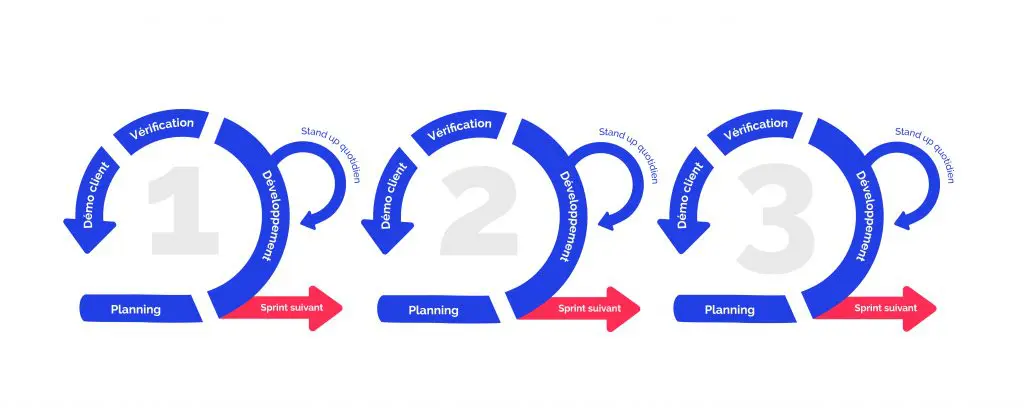
\includegraphics[width=0.7\linewidth]{Figures/Chapitre2/methode_scrum.png}
\caption{La méthode scrum}
\label{fig:ch2:scrum}
\end{figure}
Cette méthode encourage la collaboration entre les membres de l'équipe et la communication régulière avec les parties prenantes. Par conséquence, elle permet également d'améliorer continuellement le produit développé.

Dans Scrum, le projet est divisé en tâches prioritaires listées dans un Product Backlog où chaque Sprint a des objectifs spécifiques à atteindre dans un délai bien défini, généralement d'une à quatre semaines.
\subsection{Les rôles attribués dans ce projet}
La méthodologie Scrum repose principalement sur trois rôles :\\
\textbf{Product Owner }: Le rôle de Product Owner a été assuré par l’encadrant professionnel ainsi que les responsables métier de l’entreprise BIOSPHERE. Ils ont participé à la définition des besoins fonctionnels, à la priorisation des fonctionnalités et à la validation des résultats obtenus tout au long du projet.\\
\textbf{Scrum Master} : Le rôle de Scrum Master a été assuré par l’encadrante universitaire Mme Hanen Ghorbel. Ce rôle consistait à organiser les différentes phases du travail, planifier les sprints, suivre l’avancement des tâches et veiller au respect de la méthodologie Scrum.\\
\textbf{Équipe de développement} : L’équipe de développement était composée principalement de moi-même en charge du projet, responsable de :
\begin{itemize}
    \item La conception du Data Warehouse. 
    \item Le développement des workflows ETL avec n8n. 
    \item La création des tableaux de bord Power BI. 
    \item Le développement des modèles de Machine Learning.
    \item L’intégration de l’application décisionnelle.
\end{itemize}
%================= TABLE SCRUM =================


\begin{longtable}{|p{3.5cm}|p{3cm}|p{9cm}|}

\caption{Les rôles de la méthode Scrum} \\

\hline
\multicolumn{1}{|c|}{\textbf{Personne}} & 
\multicolumn{1}{c|}{\textbf{Rôle}} & 
\multicolumn{1}{c|}{\textbf{Mission}} \\
\hline
\endfirsthead

\hline
\multicolumn{1}{|c|}{\textbf{Personne}} & 
\multicolumn{1}{c|}{\textbf{Rôle}} & 
\multicolumn{1}{c|}{\textbf{Mission}} \\
\hline
\endhead
\hline
\endfoot

Encadrant professionnel et responsables métier de BIOSPHERE & Product Owner (PO) & Ils contribuent à définir les besoins fonctionnels, à prioriser les fonctionnalités et à valider les résultats obtenus tout au long du projet. \\
\hline

Mme Hanen Ghorbel & Scrum Master & Elle organise les différentes phases du travail, planifie les sprints, suit l'avancement des tâches et s'assure du respect de la méthodologie Scrum. \\
\hline

Chaima Hadj Taieb & Équipe de développement & Elle pilote la conception du Data Warehouse, le développement des workflows ETL avec n8n, la réalisation des tableaux de bord Power BI, la mise en place des modèles de Machine Learning et l'intégration de l'application décisionnelle. \\
\hline
\end{longtable}

Dans le cadre de ce projet, la méthode Scrum a été adoptée afin d’assurer une meilleure organisation des différentes phases de réalisation, notamment la conception du Data Warehouse, l’automatisation ETL, la Business Intelligence, les modèles de Machine Learning ainsi que l’intégration de l’application décisionnelle.

\section{Section 3 : Product Backlog et planification des sprints}
Le Product Backlog est un concept fondamental du cadre de travail de la méthode Scrum. Il possède l'ensemble des fonctionnalités et des tâches nécessaires pour faire la réalisation d’un projet. Les besoins se classe en User Stories pour que l’équipe puissent les prioriser et les planifier plus facilement dans chaque sprint.
\subsection{User Stories}
%================= TABLE USER STORIES =================

{\small
\renewcommand{\arraystretch}{1.2}
\setlength{\tabcolsep}{3pt}


\begin{longtable}{|p{1.8cm}|p{6cm}|p{1.8cm}|p{7cm}|}

\caption{User Stories du projet} \\

\hline
\multicolumn{1}{|c|}{\textbf{ID}} & 
\multicolumn{1}{c|}{\textbf{User Story}} & 
\multicolumn{1}{c|}{\textbf{Priorité}} & 
\multicolumn{1}{c|}{\textbf{Critères d'acceptation}} \\
\hline
\endfirsthead

\hline

\multicolumn{1}{|c|}{\textbf{ID}} & 
\multicolumn{1}{c|}{\textbf{User Story}} & 
\multicolumn{1}{c|}{\textbf{Priorité}} & 
\multicolumn{1}{c|}{\textbf{Critères d'acceptation}} \\
\hline
\endhead

\hline
\endfoot

US01 & En tant que Directeur, je veux consulter un tableau de bord consolidé des ventes, achats et stocks afin de piloter la performance globale de l'entreprise. & Haute & Affichage des 7 KPI principaux, filtre année/mois, données actualisées \\
\hline

US02 & En tant que Manager\_TN, je veux visualiser uniquement les données du site de Tunis afin de suivre la performance de mon périmètre. & Haute & Masquage automatique des données SFX, RLS actif \\
\hline

US03 & En tant que Manager\_SFX, je veux visualiser uniquement les données du site de Sfax afin de piloter mon site de manière autonome. & Haute & Masquage automatique des données TN, RLS actif \\
\hline

US04 & En tant que Décideur, je veux recevoir une alerte automatique par email pour les ruptures critiques afin de réagir avant l'impact client. & Moyenne & Déclenchement SMTP, historique sauvegardé, format standardisé \\
\hline

US05 & En tant qu'Utilisateur, je veux m'authentifier de manière sécurisée afin de garantir la confidentialité des données sensibles. & Haute & Login/mot de passe, session role-bound, déconnexion fonctionnelle \\
\hline

US06 & En tant que Responsable logistique, je veux consulter les prévisions de stock et les scores de risque afin de prioriser les réapprovisionnements. & Haute & Affichage classification + régression, tableaux produits à risque \\
\hline

US07 & En tant que Manager, je veux analyser l'historique et la répartition des fournisseurs afin de négocier les approvisionnements. & Moyenne & Top fournisseurs, répartition par site, évolution temporelle \\
\hline

US08 & En tant que Directeur, je veux suivre l'évolution des ventes par trimestre et par famille afin de détecter les tendances commerciales. & Moyenne & Graphiques temporels, filtre famille, comparaison N/N-1 \\
\hline

\end{longtable}

}

\subsection{Backlog}
Le backlog du projet a été organisé selon les principales phases de réalisation technique afin d’assurer une progression cohérente du système décisionnel, depuis la conception du Data Warehouse jusqu’à l’intégration finale dans l’application décisionnelle.\\
Le projet a été structuré en cinq sprints de durée variable, totalisant 9 semaines de développement effectif.

%================= TABLE PRODUCT BACKLOG =================

{\small
\renewcommand{\arraystretch}{1.2}
\setlength{\tabcolsep}{3pt}


\begin{longtable}{|p{3.2cm}|p{2.5cm}|p{1.5cm}|p{1.8cm}|p{7.5cm}|}

\caption{Décomposition du Product Backlog par sprint} \\

\hline
\multicolumn{1}{|c|}{\textbf{Sprint / Phase}} & 
\multicolumn{1}{c|}{\textbf{User Stories}} & 
\multicolumn{1}{c|}{\textbf{Priorité}} & 
\multicolumn{1}{c|}{\textbf{Durée}} & 
\multicolumn{1}{c|}{\textbf{Livrable attendu}} \\
\hline
\endfirsthead

\hline
\textbf{Sprint / Phase} & \textbf{User Stories} & \textbf{Priorité} & \textbf{Durée} & \textbf{Livrable attendu} \\
\hline
\endhead

\hline
\endfoot

Sprint 1 : Module Vente & US02, US03, US08 & Haute & 2 semaines & Dashboard ventes, KPI commerciaux, analyse des tendances des ventes \\
\hline

Sprint 2 : Module Achat & US07, US03, US02, US01 & Moyenne & 2 semaines & Dashboard achats, suivi des fournisseurs et indicateurs d'approvisionnement \\
\hline

Sprint 3 : Module Stock & US04, US07, US06 & Haute & 1 semaine & Dashboard stock \\
\hline

Sprint 4 : Pipeline Data Science : Prévision de stock & US02, US03, US05, US08 & Haute & 2 semaines & Modèles prédictifs :
\begin{itemize}
\item rupture de stock
\item niveau de stock
\end{itemize} \\
\hline

Sprint 5 : Application décisionnelle BIOSPHERE Decision System & US02, US03, US05 & Haute & 2 semaines & Application desktop BIOSPHERE Decision System :
\begin{itemize}
\item Authentification sécurisée (3 rôles : Directeur, Manager\_TN, Manager\_SFX) + Admin
\item Intégration des KPI BI (ventes, achats, stock)
\item Visualisation des prédictions IA
\item Système d'alertes automatisées avec notification email
\end{itemize} \\
\hline

\end{longtable}

}
\subsection{Planning de réalisation (Diagramme de Gantt)}
Le diagramme de Gantt constitue un outil essentiel dans la gestion de projet, puisqu’il permet de planifier, organiser et suivre l’ensemble des tâches à réaliser selon une chronologie bien définie. Il offre une vision claire des différentes phases du projet, des délais prévus ainsi que des dépendances entre les activités, facilitant ainsi la coordination du travail et le respect des échéances. Grâce à cet outil, l’équipe peut mieux gérer l’avancement du projet, anticiper les retards éventuels et assurer une répartition efficace des ressources. La figure 18 présente le diagramme de Gantt relatif à notre projet.
\begin{figure}[H]
\centering
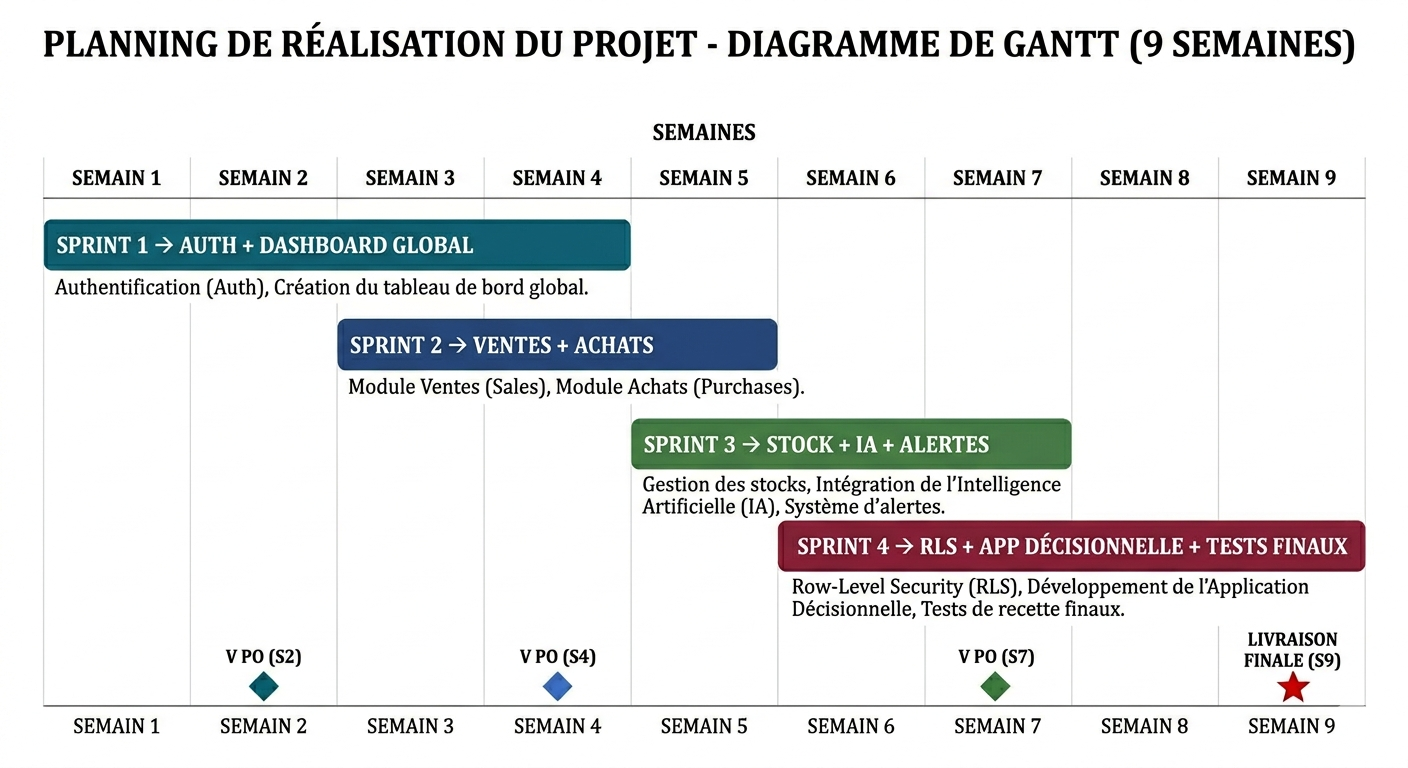
\includegraphics[width=1\linewidth]{Figures/Chapitre2/diagramme_gantt.png}
\caption{Diagramme de Gantt}
\label{fig:ch2:Gant}
\end{figure}

\section{Section 4 : Diagramme de cas d’utilisation}
\subsection{Définition d’un diagramme de cas d’utilisation}
UML, ou Unified Modeling Language, est un langage de modélisation graphique qui aide à spécifier, visualiser, construire et documenter les différents éléments d'un système d'information. Il utilise des diagrammes standardisés pour représenter de manière simple les fonctionnalités, les interactions entre les acteurs et les composants du système, sans se concentrer sur les technologies ou les langages de programmation spécifiques.\\
UML s'appuie sur divers diagrammes pour offrir une vision complète du système. Ces diagrammes peuvent illustrer les interactions entre les utilisateurs et le système, la structure du système, les processus métier, et bien plus encore. Quand on l’utilise, les équipes de développement peuvent mieux planifier et concevoir leurs systèmes, ce qui facilite la communication et réduit les risques d'erreurs ou de mauvaises interprétations.\\
Dans une perspective académique récente, ce formalisme est reconnu comme un vecteur essentiel de traçabilité des besoins, permettant de « réduire les ambiguïtés fonctionnelles dès les phases amont du projet et d’aligner la conception logicielle sur les exigences métier avant tout développement technique » \cite{Kolahdouz2024}
\subsection{Identification des acteurs et des cas}
Cette section formalise les interactions entre les utilisateurs finaux et le système décisionnel BIOSPHERE. Conformément aux standards UML, le diagramme se concentre exclusivement sur les besoins métier, en excluant toute notion d'implémentation technique (ETL, orchestration, entraînement de modèles).
\subsection{Identification des acteurs}
Trois acteurs principaux interagissent avec la solution, chacun disposant d'un périmètre d'accès strictement défini selon sa fonction organisationnelle et le principe de sécurité Row-Level Security (RLS) :
\begin{itemize}
    \item \textbf{Directeur} : Décideur stratégique disposant d'une vision globale et consolidée de l'ensemble des indicateurs, couvrant les deux sites (Tunis et Sfax) sans restriction.
    \item \textbf{Manager\_SFX }: Responsable opérationnel du site de Sfax. Son accès est automatiquement filtré pour ne restituer que les données, tableaux de bord et prévisions relatifs à son périmètre géographique.
    \item \textbf{Manager\_TN} : Responsable opérationnel du site de Tunis. Bénéficie du même niveau d'accès restreint, appliqué exclusivement aux données du site de Tunis.
\end{itemize}
\subsection{Identification des cas d'utilisation}
Les attentes métier ont été traduites en neuf cas d'utilisation principaux, répartis selon les profils utilisateurs identifiés :\\

\textbf{Cas d'utilisation associés au Directeur }
\begin{itemize}
    \item Consulter des dashboards BI GENERAL : Accès aux tableaux de bord consolidés couvrant les ventes, achats, marge et profit.
    \item Consulter Prévisions IA : Visualisation des prévisions de stock et des scores de risque de rupture à l'échelle de l'entreprise.
    \item Consulter Stock generale : Suivi des niveaux de stock, classification ABC et liste des articles en rupture pour l'ensemble du portefeuille.
\end{itemize}

\textbf{Cas d'utilisation associés au Manager\_SFX }
\begin{itemize}
    \item Consulter des dashboards BI de site de SFAX : Analyse des performances commerciales et logistiques spécifiques au site de Sfax.
    \item Consulter Prévisions IA de Sfax : Accès aux prévisions de stock et alertes de rupture propres au site de Sfax.
    \item Consulter Stock de Sfax : Consultation de l'état du stock et des indicateurs de rotation pour le site de Sfax.
\end{itemize}

\textbf{Cas d'utilisation associés au Manager\_TN}
\begin{itemize}
    \item Consulter des Dashboard BI de site de Tunis : Analyse des performances commerciales et logistiques spécifiques au site de Tunis.
    \item Consulter Prévisions IA de Tunis : Accès aux prévisions de stock et alertes de rupture propres au site de Tunis.
    \item Consulter Stock de Tunis : Consultation de l'état du stock et des indicateurs de rotation pour le site de Tunis.
\end{itemize}
\subsection{Relations et contraintes de modélisation}
Le diagramme met en évidence une contrainte fonctionnelle critique : l'authentification préalable. Chaque cas d'utilisation métier est relié au cas racine se connecter par une relation d'inclusion standardisée <<include>>.\\
Cette modélisation signifie que :
\begin{itemize}
    \item L'accès à n'importe quel tableau de bord, prévision IA ou indicateur de stock est strictement conditionné par une authentification réussie.
    \item Le cas se connecter est systématiquement exécuté en amont de toute action utilisateur, garantissant la traçabilité et la sécurité des accès.
\end{itemize}
Conformément aux bonnes pratiques UML, aucun libellé n'a été apposé sur les traits d'association, et les processus techniques en arrière-plan (workflows n8n, chargement SQL, pipelines Python) ont été volontairement exclus, car ils ne constituent pas des besoins directs des utilisateurs finaux.
\begin{figure}[H]
    \centering
    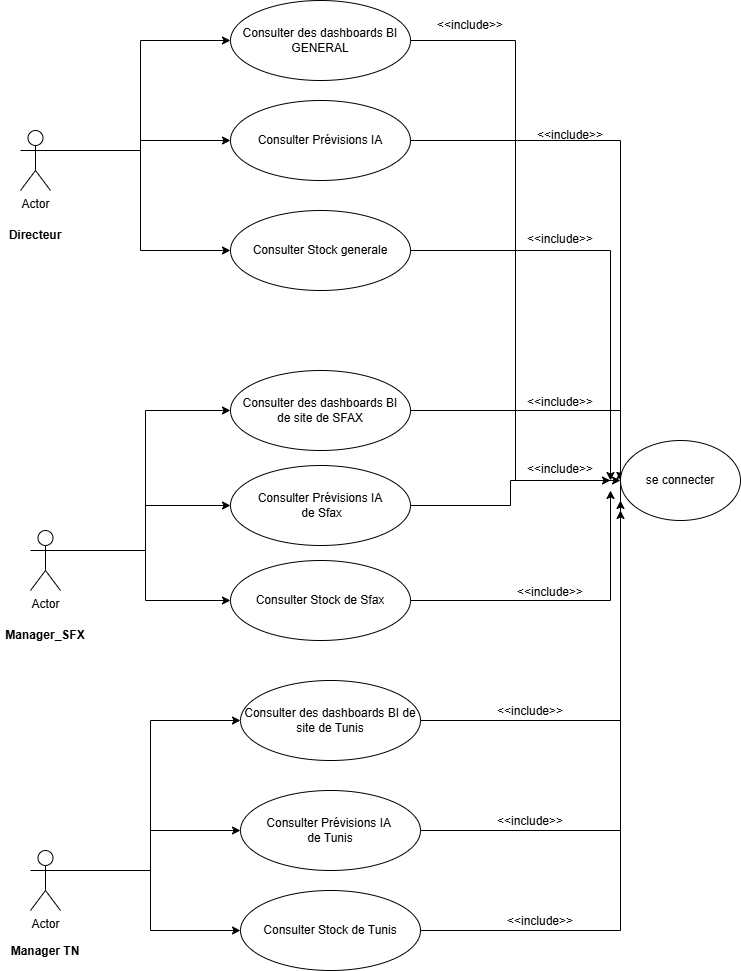
\includegraphics[width=0.9\linewidth]{Figures/Chapitre2/diagramme_cas_utilisation.png}
    \caption{Diagramme de cas d'utilisation UML du système décisionnel BIOSPHERE}
    \label{fig:UML}
\end{figure}
\section{Conclusion}
Dans ce chapitre, nous avons présenté l’approche méthodologique adoptée pour la réalisation du projet décisionnel BIOSPHERE. L’analyse des besoins a permis d’identifier les attentes fonctionnelles et techniques du système ainsi que les différents indicateurs clés de performance nécessaires au pilotage de l’activité. Ces KPI constituent une base essentielle pour l’analyse décisionnelle et le suivi des performances de l’entreprise.\\
Par ailleurs, l’adoption de la méthodologie Agile Scrum a contribué à une meilleure organisation du projet grâce à une planification progressive des tâches, une répartition claire des rôles et un suivi continu des différentes phases de développement. Les User Stories, le Product Backlog ainsi que le diagramme de Gantt ont permis de structurer efficacement les travaux réalisés tout au long du projet.
Enfin, la modélisation UML des cas d’utilisation a permis de formaliser les interactions entre les utilisateurs et le système tout en mettant en évidence les principales fonctionnalités offertes par la solution décisionnelle.\\
Les éléments présentés dans ce chapitre constituent ainsi une base méthodologique et fonctionnelle solide pour la phase suivante, consacrée à la conception technique et à l’implémentation de la solution décisionnelle et des modèles de Data Science.





\newpage


